\documentclass{standalone}
\usepackage{../../../../preamble_formulas}

\begin{document}
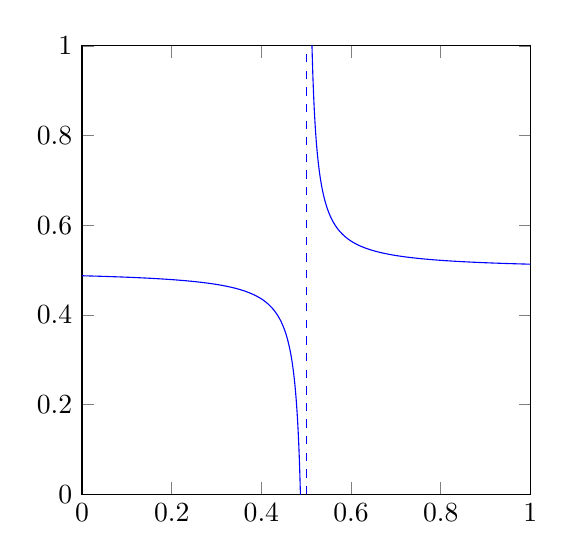
\begin{tikzpicture}
    \begin{axis}[xmin=0,xmax=1,ymin=0,ymax=1,
            axis equal image]
        \addplot [thin,samples=200,smooth,blue,domain=0:0.49] {-1/(155*(0.5-x))+0.5};
        \addplot [thin,samples=200,smooth,blue,domain=0.51:1] {1/(155*(x-0.5))+0.5};
        \draw [thin,blue,dashed] (axis cs:0.5,0) -- (axis cs:0.5,1);
    \end{axis}
\end{tikzpicture}
\end{document}